\documentclass{article}
\usepackage{fullpage}
\usepackage{biblatex}
\usepackage{graphicx}
\bibliography{refs.bib}
\setlength{\parskip}{4pt}
\setlength{\parindent}{0pt}
\title{Advanced databases: Homework 2}
\author{Leendert Dommicent and Jorn Van Loock}
\begin{document}
\maketitle
\section{Merging the ontologies}
The merging of the ontologies was done manually. Our own ontology was quite small so doing it manually seemed the best and fasted solution. In figure \ref{fig:ontology} you can find the EER diagram of our ontology from the previous assignment. Now follow the steps which we followed to merge the ontology in chronological order.
\begin{itemize}
\item We started by taking the given factbook ontology.
\item Next we added our versions of \textit{Country} and \textit{Government type} and added all the declarations of the cooresponding classes in the factbook ontology to this two classes. We also changed the decleration of our \textit{Name} property from equivalent class to superclass, because this is a shared variable who is used by many classes. This was an error in our previous ontology. We ofcourse deleted the original \textit{Country} and \textit{Government type} classes afterwards.
\item We decided to take their religion ontology because it could handle percentages and ours couldn't.
\item We replaced their object relation \textit{Government} by our relation \textit{GovernmentType}.
\item We added all our other remaining object relation, so excluding \textit{MainReligion} and \textit{hasGovernment}.
\item We added our data relations \textit{date}, \textit{id}, \textit{name} and \textit{numberOfFatalities}.
\item We changed the types of all de data properties to strings. The reason for this is given below.
\end{itemize}
The resulting ontology is the ontology we populated.
\begin{figure}
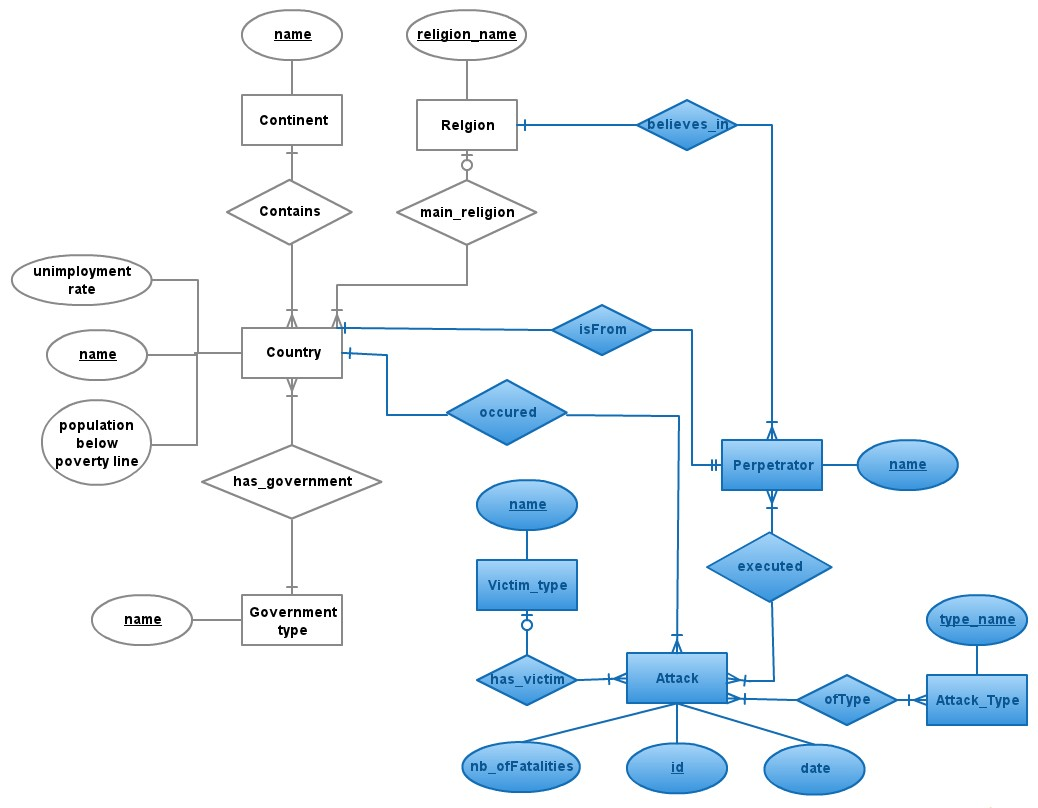
\includegraphics[width=1\textwidth]{TerroristAttacks.jpg}
\caption{Our own ontology from the first assignment}
\label{fig:ontology}
\end{figure}
\section{Automate the population}
To populate the ontologies we had to use some kind of automation because the dataset was too large to do it manually. In subsection \ref{sec:factbook} we describe how we parsed the html pages of the CIA Factbook. In subsection \ref{sec:terrorist_db} we describe how we parsed the csv file of the Terrorist Attack database. Finally in subsection \ref{sec:writ_owl} we explain how we managed to get all this data in the existing OWL ontology.
\subsection{Parsing the CIA Factbook}
\label{sec:factbook}
\subsection{Parsing the Terrorist Attack database}
\label{sec:terrorist_db}
The content of the terrorist database came in .csv format. Because .csv is a popular data format we were very confident to find a good Java parser to parse this file. We found the parser Super CSV\cite{supercsv}. Super CSV can parse .csv files and gives back a \textit{HashMap} for every record that maps the field names onto the values. Everything is parsed as a \textit{String} and handled accordingly.\par
You can find the resulting code in the class \textit{TerroristParser} in the GitHub project\cite{githubproject}.
\subsection{Writing to OWL}
\label{sec:writ_owl}
Now that we have parsed all the data we have to write it to the OWL ontology. Doing this manually by writing directly to the OWL file would be a lot of work and would be very error prone. We decided to search for a Java library that would do this for us.\par
The first Java library we tried was the one of Prot\'eg\'e. However the development of this API had stopped at the beginning of version 4 so we decided not to use this API.\par
Next we found the OWL API\cite{owlapi}. This api has a lot of features to read and write data to OWL ontologies. The only drawback was that the version for OWL 1 didn't had all the functionality we needed so we decided to use the version for OWL 2. This version didn't had any problems with reading the given OWL 1 ontology.\par
We then wrote some methods to add individuals, object relations and data relations. One drawback is that all the data properties are strings. This was the easiest solution and was good enough by our opinion for this exercise. We changed the ontology slightly by making all the data properties strings. You can find the resulting code in the class \textit{OwlHandler} in our GitHub project\cite{githubproject}.
\subsection{The final code}
\section{Conclusion}
\printbibliography
\end{document}